\section[Possible solutions]{Existing approaches}


%% TODO: move this slide to the Background section

\begin{frame}{Blockchain and smart contracts}

	\begin{exampleblock}{Smart contracts in Ethereum}
		\begin{itemize}
			\item Ethereum is a blockchain that supports \textbf{smart contracts}
			\item Smart contracts are special entities, written in the blockchain
			\begin{itemize}
				\item Execution conditions predefined and agreed on 
				\item Execute when these conditions are met
				\item Each transaction with a smart contract is a transaction in the blockchain
			\end{itemize}
		\end{itemize}
	\end{exampleblock}

\end{frame}



\begin{frame}{Existing approaches\footnote{A. Yakubov et al., "A blockchain-based PKI management framework," NOMS 2018 - IEEE/IFIP Network Operations and Management Symposium, Taipei, 2018, pp. 1-6.}}
\begin{columns}
\begin{column}{0.48\textwidth}
	\begin{exampleblock}{Ethereum smart contracts}
%	\begin{exampleblock}{Ethereum smart contracts}
		\begin{itemize}
			\item Each certification authority has \textbf{smart contracts} that store a list of issued certificates and a revocation list
			\item Specific format for certificates: \textbf{hybrid certificates}
		\end{itemize}
	\end{exampleblock}
\end{column}
\begin{column}{0.48\textwidth}
	\begin{center}
		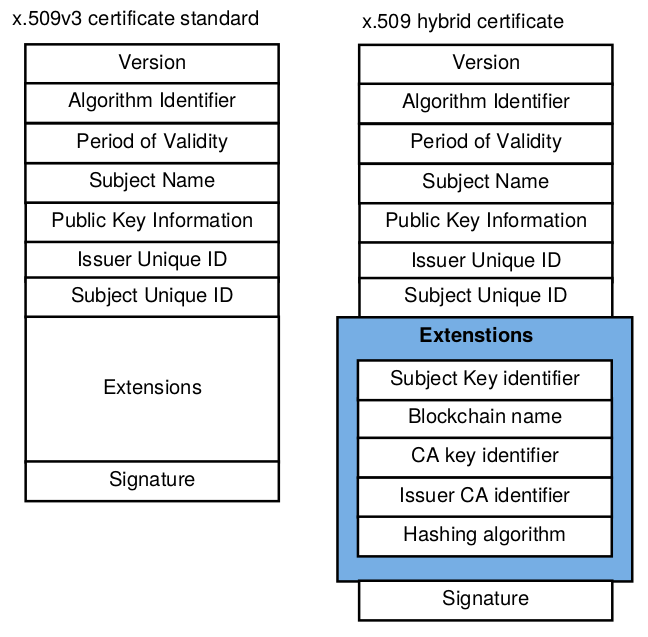
\includegraphics[scale=0.2]{figs/article_pki_blockchain.png}
	\end{center}
\end{column}
\end{columns}
\end{frame}


%\begin{frame}{Existing approaches}
%
%	\begin{exampleblock}{Ethereum smart contracts\footnote{A. Yakubov et al., "A blockchain-based PKI management framework," NOMS 2018 - IEEE/IFIP Network Operations and Management Symposium, Taipei, 2018, pp. 1-6.}}
%		\begin{itemize}
%			\item Each certification authority has \textbf{smart contracts} that store a list of issued certificates and a revocation list
%			\item Specific format for certificates: \textbf{hybrid certificates}
%		\end{itemize}
%	\end{exampleblock}
%	
%	\begin{center}
%		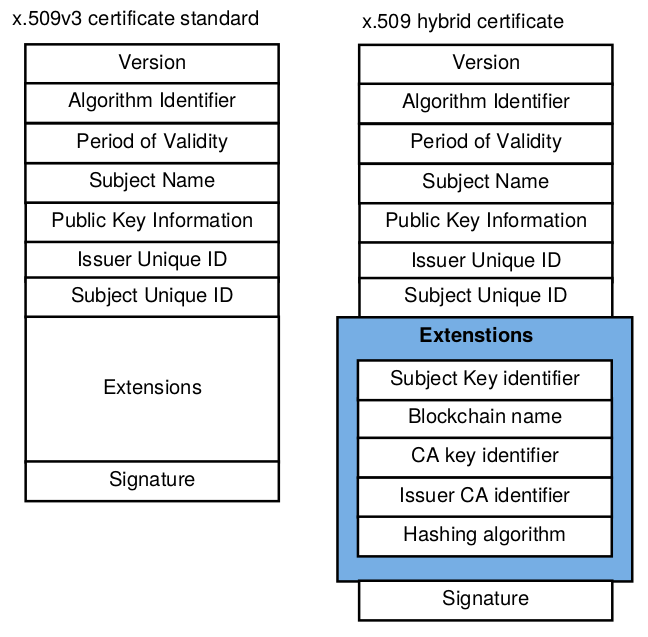
\includegraphics[scale=0.3]{figs/article_pki_blockchain.png}
%	\end{center}
%
%\end{frame}

\begin{frame}{Existing approaches}
	\begin{exampleblock}{Data fields in Bitcoin-based blockchains}
		\begin{itemize}
			\item Special \textbf{OP\_RETURN} field can contain arbitrary data
			\begin{itemize}
				\item Many applications, such as Intellectual Property
			\end{itemize}
			\item Bitcoins: maximum size of 80 bytes
			\item Several blockchains could be used, such as Bitcoin or Namecoin
		\end{itemize}
	\end{exampleblock}
\end{frame}







